\documentclass[a4paper, 11pt]{article}

\usepackage{geometry}
\usepackage{amsmath,amssymb}
\usepackage{ifthen}

\usepackage{tikz}
\usetikzlibrary{calc,math}

\makeatletter
\pgfdeclareshape{oplus}{%{{{
  \inheritsavedanchors[from=circle]
  \inheritanchorborder[from=circle]
  \foreach \s in {center,mid,base,text, north,south,west,east,
                  mid west,mid east,base west,base east,
                  north west,south west,north east,south east} {
    \inheritanchor[from=circle]{\s}
  }
  \backgroundpath{%
    \pgfutil@tempdima=\radius%
    \pgfmathsetlength{\pgf@xb}{\pgfkeysvalueof{/pgf/outer xsep}}%  
    \pgfmathsetlength{\pgf@yb}{\pgfkeysvalueof{/pgf/outer ysep}}%  
    \ifdim\pgf@xb<\pgf@yb%
      \advance\pgfutil@tempdima by-\pgf@yb%
    \else%
      \advance\pgfutil@tempdima by-\pgf@xb%
    \fi%
    \pgfpathcircle{\centerpoint}{\pgfutil@tempdima}%
    % north-south
    \centerpoint\advance\pgf@y by\radius  \pgf@xa=\pgf@x \pgf@ya=\pgf@y
    \centerpoint\advance\pgf@y by-\radius \pgf@xb=\pgf@x \pgf@yb=\pgf@y
    \pgfpathmoveto{\pgfpoint{\pgf@xa}{\pgf@ya}}
    \pgfpathlineto{\pgfpoint{\pgf@xb}{\pgf@yb}}
    % east-west
    \centerpoint\advance\pgf@x by\radius  \pgf@xa=\pgf@x \pgf@ya=\pgf@y
    \centerpoint\advance\pgf@x by-\radius \pgf@xb=\pgf@x \pgf@yb=\pgf@y
    \pgfpathmoveto{\pgfpoint{\pgf@xa}{\pgf@ya}}
    \pgfpathlineto{\pgfpoint{\pgf@xb}{\pgf@yb}}
  }
}%}}}
\makeatother
\tikzset{op/.style={draw, fill=none, minimum size=1.25ex, inner sep=0pt}}
\tikzset{opxor/.style={op, shape=oplus}}
\tikzset{opand/.style={op, rectangle, rounded corners=2pt, minimum height=3ex}}
\tikzset{oprot/.style={op, rectangle, rounded corners=2pt, inner sep=2pt, minimum width=3ex, font=\scriptsize}}
\tikzset{optee/.style={shape=circle, fill, draw, inner sep=0pt, minimum size=2pt}}
\tikzset{next/.style={->, >=latex}}

\newcommand{\cipher}[1]{\textsf{#1}}

\newif\ifsubstates\substatesfalse


\begin{document}

\noindent
2 approximations for $S^{2,2}_{0}$:
\begin{align*}
  S^{2,2}_0 &= C^0_{27} \oplus C^1_{0, 8, 26} \oplus C^2_{7,13,31} \oplus C^3_{12} \tag{corr. $2^{-7}$} \\
  S^{2,2}_0 &= C^1_{2} \oplus C^2_{1,7,15,27} \oplus C^3_{6,14,20} \oplus
  C^4_{19} \tag{corr. $2^{-9}$} \\
\intertext{Combined ciphertext-only approximation:}
  0 &= C^0_{27} \oplus C^1_{0, 2, 26, 8} \oplus C^2_{1,13,15,27,31} \oplus
  C^3_{6,12,14,20} \oplus C^4_{19} \tag{corr. $2^{-16}$}
\end{align*}

\begin{figure}
  \substatesfalse
  % \substatesfalse to label state words and/or masks
  \centering
  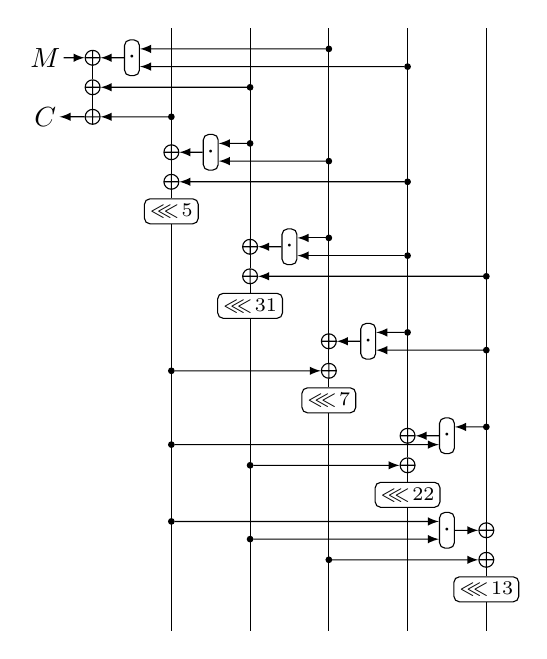
\begin{tikzpicture}[xscale=1.0,yscale=1.5]%{{{
  \ifsubstates \pgfmathsetmacro{\roundsep}{1.25}
  \else        \pgfmathsetmacro{\roundsep}{0.80} \fi
  \pgfmathsetmacro{\opoffset}{.1}

  \ifsubstates
    \foreach \r in {-2,...,4} {
      \foreach \w in {0,...,4} {
        \draw[thick] (\w-.5,-\r*\roundsep) -- ++(0,-.25);
        \node[minimum width=1*1.0cm,minimum height=.25*1.5cm, inner sep=0pt] (W\r\w) at (\w,-\r*\roundsep-.125) {};
      }
      \draw[thick] (-.5,-\r*\roundsep) node[below left, inner sep=0pt, xshift=-3pt] {$S_{\r,*}^{\r}$} rectangle ++(5,-.25);
    }
    \node[minimum width=1*1.0cm,minimum height=.25*1.5cm, inner sep=0pt] (W-1-1) at (-1,--1*\roundsep-.125) {};
    \node[minimum width=1*1.0cm,minimum height=.25*1.5cm, inner sep=0pt] (W-2-1) at (-2,--1*\roundsep-.125) {};
  \else
    \foreach \r in {-1,...,4} {
      \foreach \w in {0,...,4} {
        \coordinate (W\r\w) at (\w,-\r*\roundsep-.125);
      }
    }
    \foreach \w in {0,...,4} {
      \coordinate (W-2\w) at (\w,--2.375*\roundsep-.125);
    }
    \coordinate (W-1-1) at (-1,--1*\roundsep-.125);
    \coordinate (W-2-1) at (-2,--1*\roundsep-.125);
  \fi

  \foreach \r/\rot in {-1/0,0/5,1/31,2/7,3/22,4/13} { % round
    \ifthenelse{\equal{\r}{-1}}{
      \pgfmathsetmacro{\txorx}{int(mod(\r+2,5))}
      \pgfmathsetmacro{\tanAx}{int(mod(\r+4,5))}
      \pgfmathsetmacro{\tanBx}{int(mod(\r+3,5))}
      \pgfmathsetmacro{\tlllx}{int(mod(\r+1,5))}
    }{
      \pgfmathsetmacro{\txorx}{int(mod(\r+3,5))}
      \pgfmathsetmacro{\tanAx}{int(mod(\r+2,5))}
      \pgfmathsetmacro{\tanBx}{int(mod(\r+1,5))}
    }
    \pgfmathsetmacro{\rprev}{int(\r-1)}
    \ifthenelse{\equal{\r}{-1}}%
    { \node[opxor] (lll\r) at ($(W\r\r) +(0,\opoffset+.25)$)  {}; }%
    { \node[oprot] (lll\r) at ($(W\r\r) +(0,\opoffset+.25)$)  {$\lll\!\rot$}; }
      \node[opxor] (xor\r) at ($(W\r\r) +(0,\opoffset+.50)$)  {};
      \node[opxor] (xnd\r) at ($(W\r\r) +(0,\opoffset+.75)$)  {};
    \ifthenelse{\equal{\r}{4}}
    { \node[opand] (and\r) at ($(W\r3) +(.5,\opoffset+.75)$)  {$\cdot$}; }
    { \node[opand] (and\r) at ($(W\r\r) +(.5,\opoffset+.75)$) {$\cdot$}; }
    \ifthenelse{\equal{\r}{-1}}%
    { \node[inner sep=1pt] (M) at ($(xnd\r) +(-.6,0)$) {$M$};
      \node[inner sep=1pt] (C) at ($(lll\r) +(-.6,0)$) {$C$};
      \draw[next] (M) -- (xnd\r);
      \draw[next] (lll\r) -- (C);
      \coordinate[optee] (tlll\r) at ($(W\r\tlllx) +(0,\opoffset+.25)$); }{}
      \coordinate[optee] (txor\r) at ($(W\r\txorx) +(0,\opoffset+.50)$);
      \coordinate[optee] (tanA\r) at ($(W\r\tanAx) +(0,\opoffset+.675)$);
      \coordinate[optee] (tanB\r) at ($(W\r\tanBx) +(0,\opoffset+.825)$);

    \ifthenelse{\equal{\r}{-1}}%
    { \draw[next] (tlll\r) -- (lll\r); }{}
      \draw[next] (txor\r) -- (xor\r);
    \ifthenelse{\tanAx < \r}%
    { \draw[next] (tanA\r) -- (tanA\r-|and\r.west); }%
    { \draw[next] (tanA\r) -- (tanA\r-|and\r.east); }
    \ifthenelse{\tanBx < \r}%
    { \draw[next] (tanB\r) -- (tanB\r-|and\r.west); }%
    { \draw[next] (tanB\r) -- (tanB\r-|and\r.east); }
    \draw[next] (and\r) -- (xnd\r);
    \draw[    ] (xnd\r) -- (xor\r);
    \draw[    ] (xor\r) -- (lll\r);

    \foreach \w in {0,...,4} {
      \ifthenelse{\equal{\w}{\r}}{
        \draw (W\rprev\w) -- (xnd\r);
        \draw (lll\r) -- (W\r\w);
      }{
        \draw (W\rprev\w) -- (W\r\w);
      }
    }
  }
  \end{tikzpicture}%}}}
  \caption{\cipher{MiniMorus} state update function (1 step = 5 rounds).}
  \label{fig:minimorus}
\end{figure}

\end{document}
